% \documentclass[CJKutf8, 10pt, handout]{beamer}
\documentclass[CJKutf8, 10pt]{beamer}
\usetheme[
%%% options passed to the outer theme
%    hidetitle,           % hide the (short) title in the sidebar
%    hideauthor,          % hide the (short) author in the sidebar
%    hideinstitute,       % hide the (short) institute in the bottom of the sidebar
%    shownavsym,          % show the navigation symbols
%    width=2cm,           % width of the sidebar (default is 2 cm)
%    hideothersubsections,% hide all subsections but the subsections in the current section
%    hideallsubsections,  % hide all subsections
%    right                % right of left position of sidebar (default is right)
]{Aalborg}
  
% If you want to change the colors of the various elements in the theme,
% edit and uncomment the following lines.
% Change the bar and sidebar colors:
%\setbeamercolor{Aalborg}{fg=red!20,bg=red}
%\setbeamercolor{sidebar}{bg=red!20}
% Change the color of the structural elements:
%\setbeamercolor{structure}{fg=red}
% Change the frame title text color:
%\setbeamercolor{frametitle}{fg=blue}
% Change the normal text color background:
\setbeamercolor{normal text}{bg=gray!6}

\usepackage{subfigure}
\usepackage{CJKutf8}
\usepackage{color}
\usepackage{pgf}
\usepackage{graphicx}
\usepackage{fancybox}
\usepackage[utf8]{inputenc}
\usepackage[english]{babel}
\usepackage[T1]{fontenc}
% ... or whatever. Note that the encoding and the font should match.
% If T1 does not look nice, try deleting the line with the fontenc.
\usepackage{lmodern} %optional
\usepackage{listings}
\usepackage{wasysym}
\graphicspath {{figure/}}
\hypersetup{pdfpagemode={FullScreen}}

% % % % % % 缩写  %%%%%%%%%
\newcommand{\PM}{\ PM$_{10}\ $}
\newcommand{\SO}{\ SO$_{2}\ $}
\newcommand{\NO}{\ NO$_{2}\ $}
\newcommand{\uml}{\mu\hspace{-0.03cm}g$/$m$^{3}$}

%%%%%%%% User Specified Commands %%%%%%%%
\setbeamercolor{alerted text}{fg=red!2!green!35!blue}
\renewcommand{\baselinestretch}{1.3} \normalsize}   % % % % 设置行间距
\newenvironment{boxalertenv}{\begin{altenv}%
  {\usebeamertemplate{alerted text begin}\usebeamercolor[fg]
    {alerted text}\usebeamerfont{alerted text}\colorbox{bg}}
  {\usebeamertemplate{alerted text end}}{\color{.}}{}}{\end{altenv}}
\newcommand<>{\boxalert}[1]{{%
  \begin{boxalertenv}#2{#1}\end{boxalertenv}%
}}

\def\hilite<#1>{%
  \temporal<#1>{\color{gray}}{\color{red!2!green!35!blue}}%
    {\color{blue!25}}}

\definecolor{listinggray}{gray}{0.9}
\definecolor{lbcolor}{rgb}{0.9,0.9,0.9}


\lstset{
	language=C,
	captionpos=b,
	tabsize=4,
	frame=lines,
	keywordstyle=\color{blue},
	commentstyle=\color{darkgreen},
	stringstyle=\color{red},
	breaklines=true,
	showstringspaces=false,
	basicstyle=\footnotesize,
	emph={label}
	}

%%%%%%%% 设置字号 %%%%%%%%
\newcommand{\chuhao}{\fontsize{42pt}{\baselineskip}\selectfont}
\newcommand{\xiaochuhao}{\fontsize{36pt}{\baselineskip}\selectfont}
\newcommand{\yihao}{\fontsize{28pt}{\baselineskip}\selectfont}
\newcommand{\erhao}{\fontsize{21pt}{\baselineskip}\selectfont}
\newcommand{\xiaoerhao}{\fontsize{18pt}{\baselineskip}\selectfont}
\newcommand{\sanhao}{\fontsize{15.75pt}{\baselineskip}\selectfont}
\newcommand{\sihao}{\fontsize{14pt}{\baselineskip}\selectfont}
\newcommand{\xiaosihao}{\fontsize{12pt}{\baselineskip}\selectfont}
\newcommand{\wuhao}{\fontsize{10.5pt}{\baselineskip}\selectfont}
\newcommand{\xiaowuhao}{\fontsize{9pt}{\baselineskip}\selectfont}
\newcommand{\liuhao}{\fontsize{7.875pt}{\baselineskip}\selectfont}
\newcommand{\xiaoliuhao}{\fontsize{6.05pt}{\baselineskip}\selectfont}
\newcommand{\qihao}{\fontsize{5.25pt}{\baselineskip}\selectfont}

\AtBeginSection[]
{
\begin{frame}[shrink]
\begin{CJK}{UTF8}{gbsn}
  \frametitle{目录}
  \CJKfamily{you}{\tableofcontents[%
 		currentsection, % causes all sections but the current to be shown in a semi-transparent way.
% 		currentsubsection, % causes all subsections but the current subsection in the current section to ...
% 		hideallsubsections, % causes all subsections to be hidden.
 		hideothersubsections, % causes the subsections of sections other than the current one to be hidden.
% 		part=, % part number causes the table of contents of part part number to be shown
%		pausesections, % causes a \pause command to be issued before each section. This is useful if you
% 		pausesubsections, %  causes a \pause command to be issued before each subsection.
% 		sections={ overlay specification },
  ]}
\end{CJK}
\end{frame}
}

\begin{document}
\begin{CJK}{UTF8}{song}

\title[空气污染与R软件]% optional, use only with long paper titles
{\erhao 空气污染与R软件  \\[2ex]}
\author[张兵] % optional, use only with lots of authors
{
\vspace{-0.7cm}
\textcolor[rgb]{0.00, 0.41, 0.66}{\sihao 张兵}  \\
\vspace{0.3cm}
\textcolor[rgb]{0.00, 0.41, 0.66}{Email: zhangbing4502431@outlook.com} \\
\vspace{0.3cm}
\textcolor[rgb]{0.00, 0.41, 0.66}{Homepage: \href{http://spatial-r.github.io/}{http://spatial-r.github.io/}}
% \href{mailto:haipingf@gmail.com}{{\tt haipingf@gmail.com}}
}


% - Give the names in the same order as they appear in the paper.
% - Use the \inst{?} command only if the authors have different
%   affiliation. See the beamer manual for an example

%specify some optional logos
% placed in the upper left/right corner
%\pgfdeclareimage[height=1.3cm]{mainlogo}{CDC.png} 
%\logo{\pgfuseimage{mainlogo}}
% placed in the lower left/right corner if the \pgfuseimage{minilogo} command is
% uncommented in the \institute command below.
%\pgfdeclareimage[height=0.6cm]{minilogo}{CDC.pdf} 

\institute[
  %{\pgfuseimage{minilogo}}\\ %insert a company or department logo
    Zhejiang Provincial Center for
    Disease Control and Prevention
] % optional - is placed in the bottom of the sidebar on every slide
{%
\textcolor[rgb]{0.07, 0.31, 0.60}{
  \wuhao 浙江省疾病预防控制中心\\[2ex]}
  
  % there must be an empty line above this line - otherwise some unwanted space is added
  % between the university and the country (I do not know why;( )
}
% \date{\today}
\date{\textcolor[rgb]{0.00, 0.41, 0.46}{2014 年 12 月 6 日}}

% the titlepage
% the plain option removes the sidebar and header from the title page
\begin{frame}[plain] 
  \titlepage
\end{frame}
%%%%%%%%%%%%%%%%

%%%%%%%%%%%%%%%%%%%%%%%%%%%%%%%%%%%%%%%%%%%%%%%%%%%%%%%%%%%%
\section{空气污染--简介}
\subsection{空气污染}
\begin{frame}{空气污染}
\begin{itemize}
  \item  空气污染(Air pollution)通常是指由于人类活动或自然过程引起某些物质进入大气中,
  呈现出足够的浓度,达到足够的时间,并因此危害了人类的舒适、健康和福利或环境的现象。
  \item   空气污染的主要来源是工业、锅炉、交通运输等。
 \end{itemize}
 \begin{figure}
 \centering
 \subfigure[雾中有太极]{
 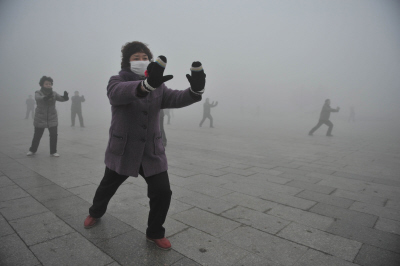
\includegraphics[width=0.45\textwidth,heigth=0.3\textwidth]{flog2.jpg}
 }
 \subfigure[长跑须防毒]{
 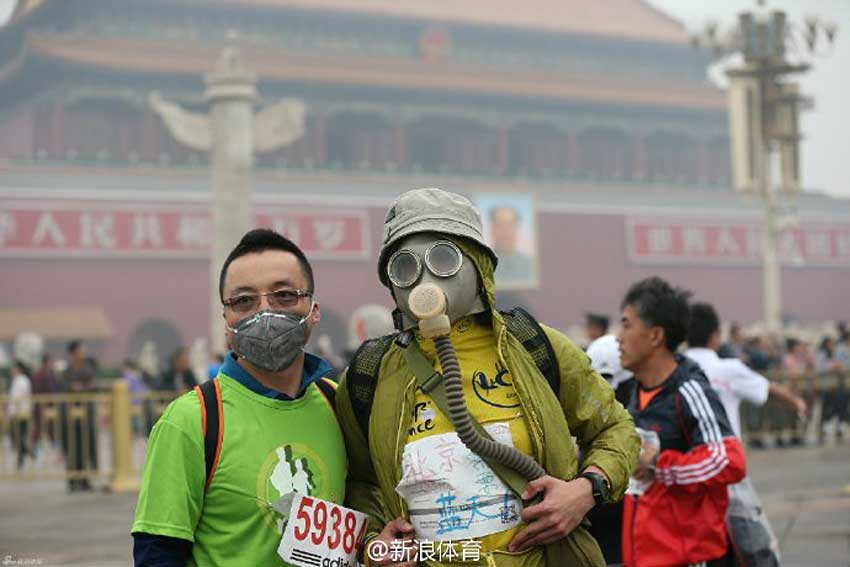
\includegraphics[width=0.45\textwidth,heigth=0.3\textwidth]{flog1.jpg}
 }
  \end{figure}
 \end{frame}

%%%%%%%%%%%%%%%%
\subsection{监测指标}
\begin{frame}{监测指标}
空气质量标准(GB: 3095-2012),监测指标及其浓度限值:\\
\begin{figure}
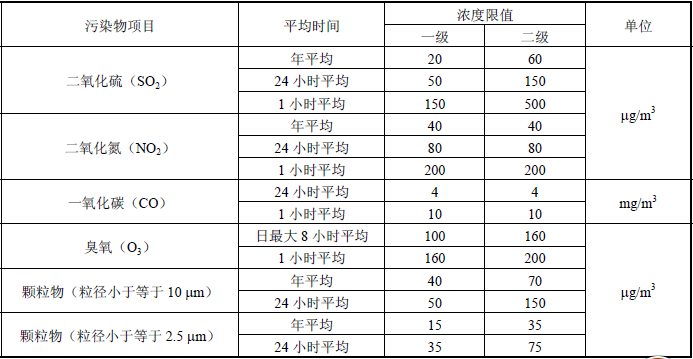
\includegraphics[width=0.8\textwidth,heigth=0.9\textwidth]{stardart.png}
\end{figure}
\begin{itemize}
\item 一级标准适合于自然保护区、风景名胜区和其他需要特殊保护的区域。
\item   二级标准适合与居民区、商业交通居民混合区、文化区、工业区和农村地区。
\end{itemize}
\end{frame}

\subsection{空气质量指数}
\begin{frame}{空气质量指数}
\begin{itemize}
\item 空气质量指数(Air Quality Index, AQI)是定量描述空气质量状况的非线性无量纲指数,数值越大,说明空气污染状况越严重。其计算方式为:
\begin{align}
AQI=max\{IAQI_{1},IAQI_{2},IAQI_{3},...,IAQI_{n}\}
\end{align}
式中:IAQI为空气质量分指数;n为污染物项目。
\item  污染物项目P的空气质量分指数(IAQI$_{p}$)的计算方式如下:
\begin{align}
IAQI_{p}=\frac{IAQI_{Hi}-IAQI_{Lo}}{BP_{Hi}-BP_{Lo}}(C_{p}-BP_{Lo})+IAQI_{Lo}
\end{align}
式中:$C_{p}$为污染物P的浓度;$BP_{Hi}$和$BP_{Lo}$分别为国家环境保护标准HJ633-2012中与$C_{p}$相近的污染物浓度的高位值和低位值;$IAQI_{Hi}$和$IAQI_{Lo}$分别是与$BP_{Hi}$和$BP_{Lo}$相对应的空气质量分指数。
\end{itemize}
\end{frame}

%%%%%%%%%%%%%%%%%%%%%%%%%%%%%%%%%%%%%%%%%%%%%%%%%%%%%%%%%%%%
\section{空气污染--数据获取}
\subsection{数据来源}
\begin{frame}{数据来源}
\begin{itemize}
\item  \href{http://datacenter.mep.gov.cn/}{\alert{国家环保局数据中心}}: 城市逐日空气质量指数数据(起始时间为2014年1月1日)
\vspace{0.2cm}
\item  各省及各市的环境保护局,如\href{http://www.whepb.gov.cn/airInfoView.jspx?listPath=hbHjjc}{\alert{武汉市环保局}},10个国控点各个污染物分指数数据。
\vspace{0.2cm}
\item  数据存放在相应GIS平台上,如\href{http://www-app.gdepb.gov.cn/EQpubplatform/Default.aspx}{\alert{广东省环境信息综合发布平台}}及\href{http://aqicn.org/city/beijing/cn/}{\alert{亚洲空气质量公布平台}}。
\vspace{0.2cm}  
\item  某些网站会无偿公开空气污染数据的API接口,如\href{http://www.pm25.in/api_doc}{\alert{PM25.in}}.
\vspace{0.2cm}
 \item 公共信息平台上,如\href{http://weibo.com/637578234}{\alert{微博AQI}}及\href{http://weibo.com/hzpm}{\alert{微博PM$_2_._5$}}。
\end{itemize}
\end{frame}

\subsection{获取方式}
\begin{frame}{数据获取--1}
总的原则:利用\href{http://cran.r-project.org/web/packages/RCurl/index.html}{\alert{RCurl}}或(和)\href{http://cran.r-project.org/web/packages/XML/index.html}{\alert{XML}}解析网页,提取数据。\\
\hspace{0.5cm}网页中有历史数据,直接用代码读取;\\
\hspace{0.5cm}实时更新的网页,在R软件中设置循环,整点读取数据。
\begin{itemize}
\vspace{0.3cm}
\item 国家环保局数据中心,代码如下:  \\
\begin{figure}
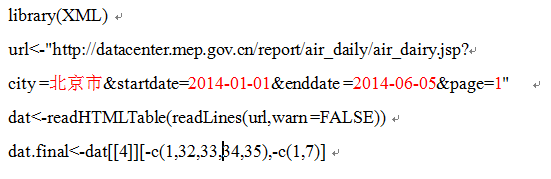
\includegraphics[width=0.8\textwidth,heigth=0.9\textwidth]{code1.png}
\end{figure}
\item 改变city、startdate、enddate和page参数值,进而获取不同城市在不同时间段空气质量指数数据。
\end{itemize}
\end{frame}

\begin{frame}{数据获取--2}
\begin{itemize}
\item  广东省环境信息综合发布平台,{代码}{\footnote{感谢肖楠大神}}如下:
\begin{figure}
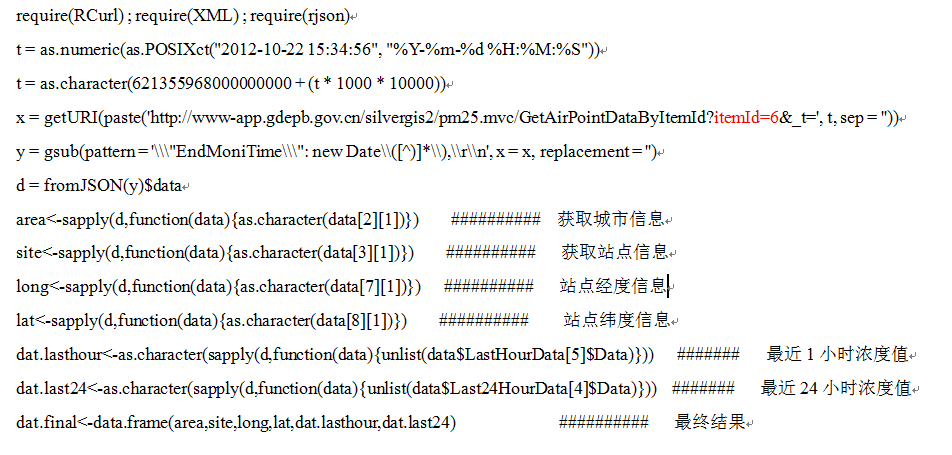
\includegraphics[width=0.9\textwidth,heigth=0.9\textwidth]{code2.png}
\end{figure}
\vspace{-0.3cm}
\item 改变itemId参数的值,即可获得其他空气污染物数据。
\end{itemize}
\vspace{-0.3cm}
\begin{table}
\qihao
\begin{tabular}{|c|c|c|c|c|c|c|c|c|}
\hline
itemId & 1& 2& 3& 4 & 5 & 6  & 7 & 8  \\
\hline
指标 & SO$_{2}$ & NO$_{2}$ &O$_{3}$1h & O$_{3}$8h & PM$_{10}$ & PM$_{2.5}$ & AQI & CO \\
\hline
\end{tabular}
\end{table}
\end{frame}

\begin{frame}{数据获取--3}
Pm25.in 网页提供了国家环保局数据的API接口(相关说明可参见\href{http://www.pm25.in/api_doc}{\alert{这}})。\\
获取全国所有站点空气质量数据的示例代码如下:
\begin{figure}
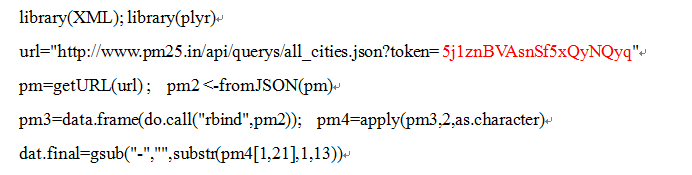
\includegraphics[width=0.9\textwidth,heigth=0.9\textwidth]{code3.png}
\end{figure}
需注意两点:
\begin{itemize}
\item  需要申请密钥,上述代码中的密钥是公钥。
\item  API调用次数限制:1.10和1.11每小时15次、1.12每小时5次、1.13每小时15次,其余每小时500次。
\end{itemize}
\end{frame}


\section{空气污染--描述性分析}

\begin{frame}[plain]
\begin{center}
\begin{figure}
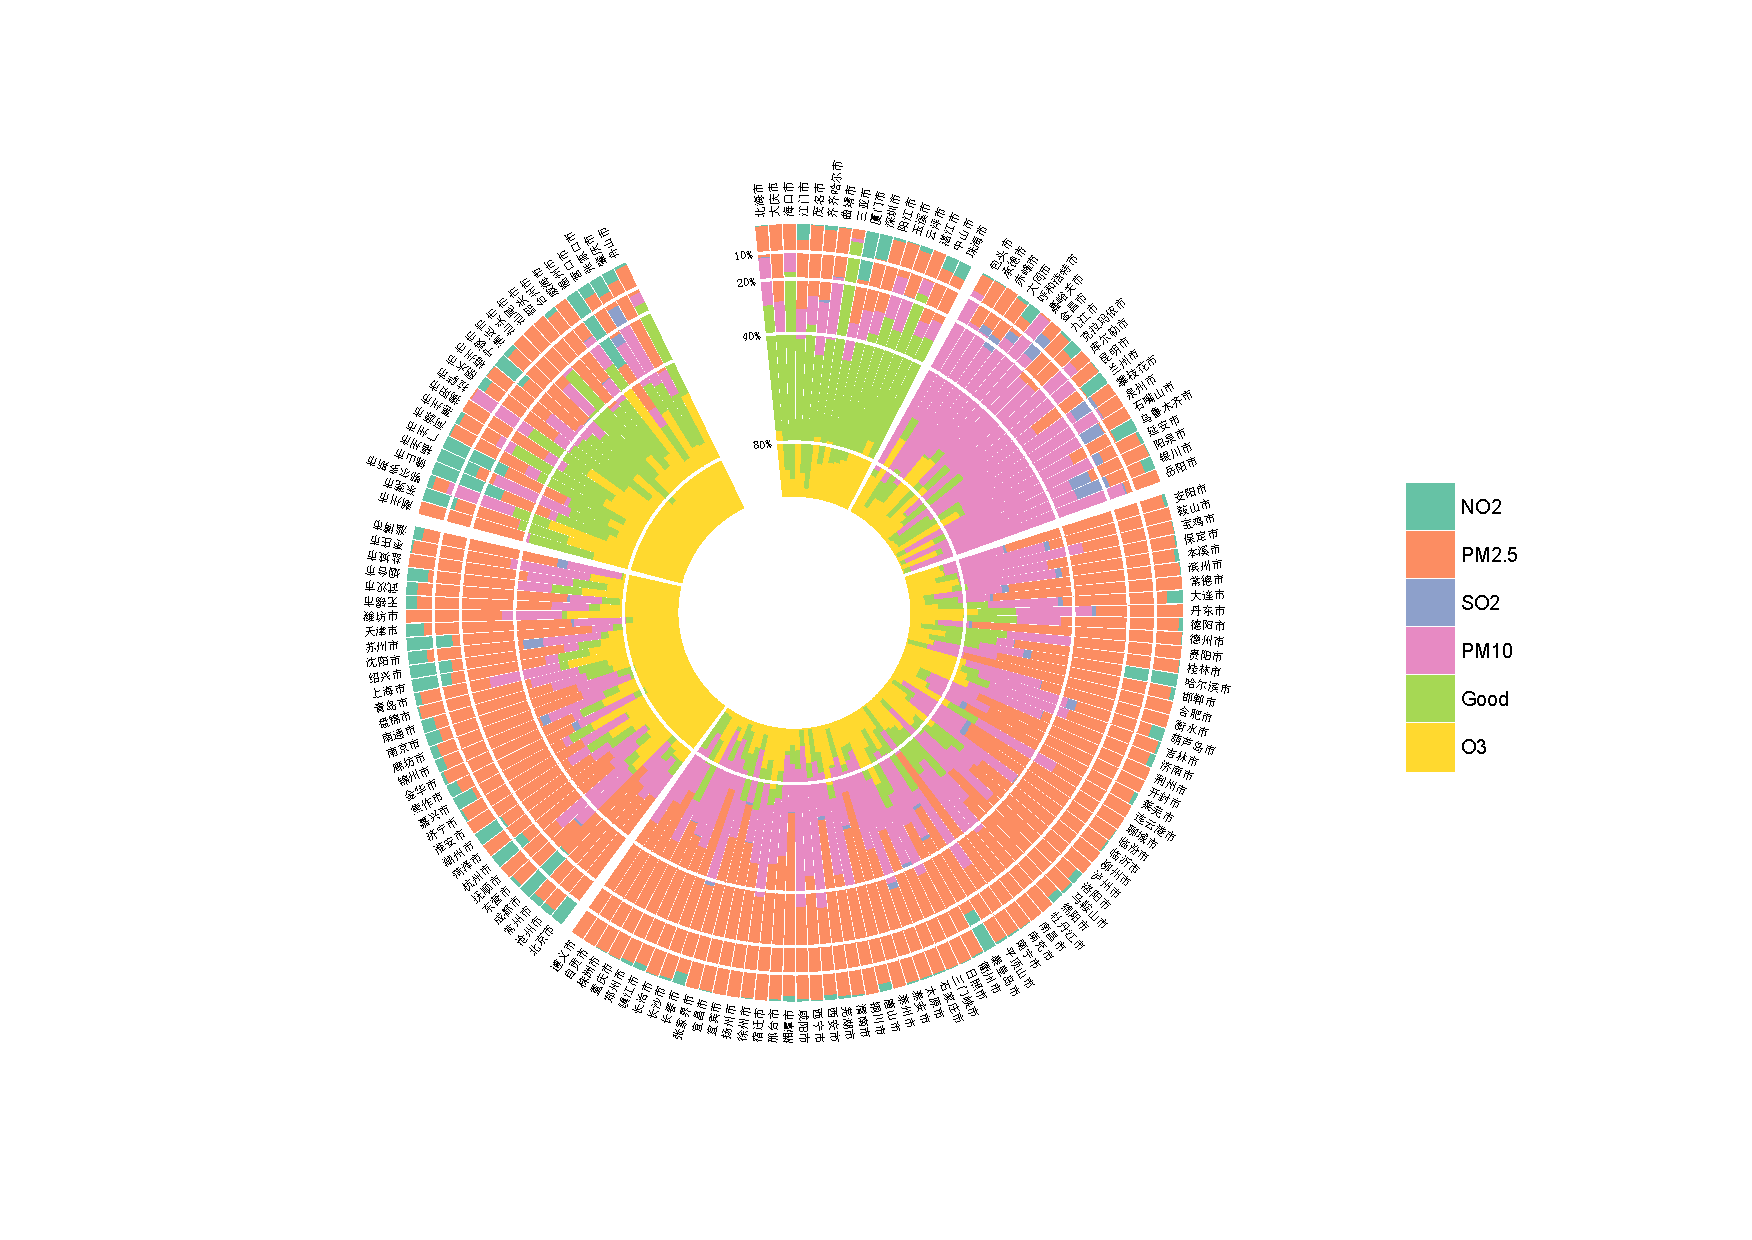
\includegraphics[width=0.9\textwidth,heigth=0.9\textwidth]{Mpollutant.pdf}
\end{figure}
全国空气质量一览,PM$_{10}$、PM$_{2.5}$和臭氧是主要的污染物!
\end{center}
\end{frame}

\subsection{时间维度}
\begin{frame}{日历图: openair }
上海市PM$_{2.5}$日均浓度
 \begin{figure}
 \centering
 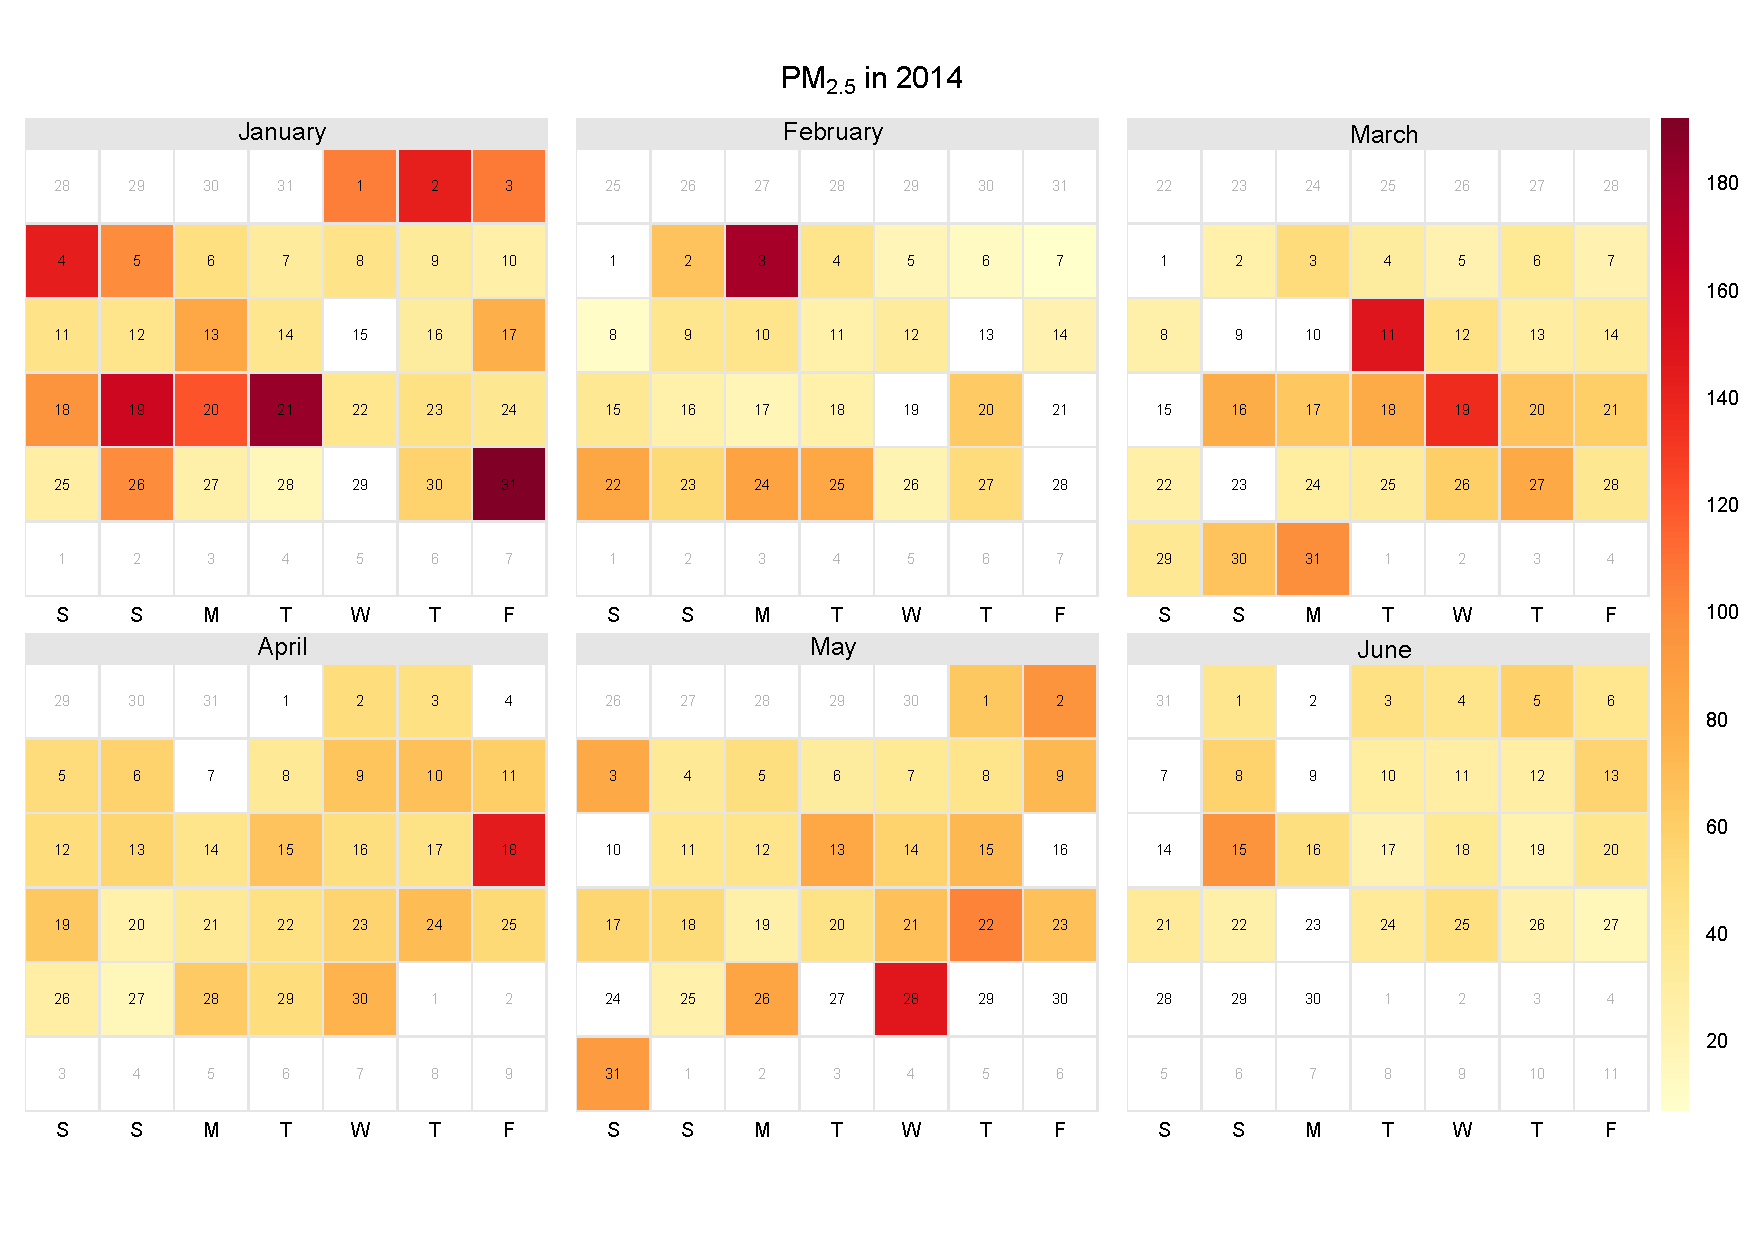
\includegraphics[width=\textwidth,heigth=\textwidth]{pm25.pdf}
  \end{figure}
  \end{frame}

\subsection{空间维度}
\begin{frame}{空间维度: ggplot2和automap}
2014年11月11日PM$_{2.5}$日均浓度:
\begin{figure}
 \subfigure[日均浓度]{
 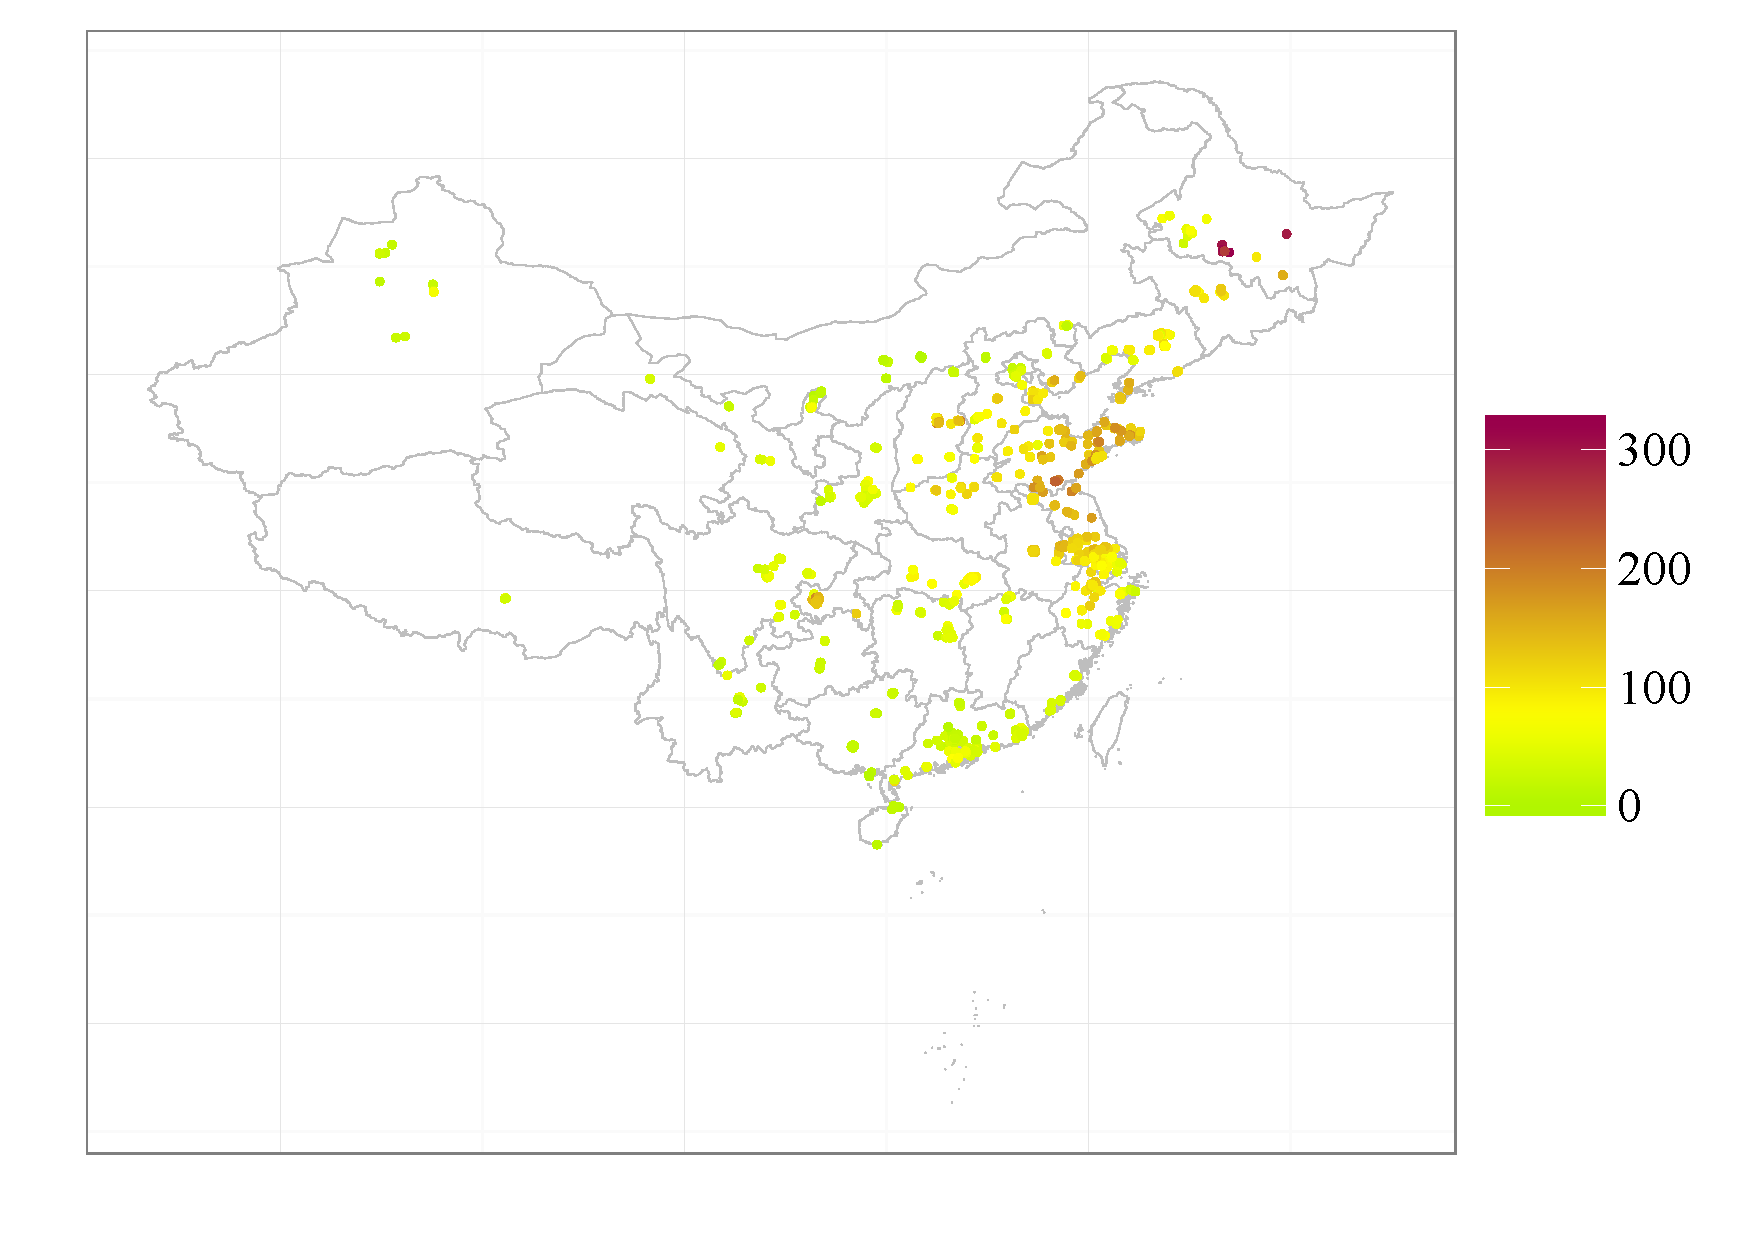
\includegraphics[width=0.45\textwidth,heigth=0.3\textwidth]{11pm25.pdf}
 }
 \subfigure[空间插值]{
 \includegraphics[width=0.45\textwidth,heigth=0.3\textwidth]{interpretation.pdf}
 }
 \end{figure}
 近45.6\%的监测站点PM$_{2.5}$日均浓度超过了空气质量二级标准限值,主要集中在山东和江苏地区。光棍相亲需慎重,既面临被拒的风险,也面临着空气污染的毒害!
\end{frame}

\section{空气污染--健康效应}
\subsection{研究方法}
\begin{frame}{研究方法}
空气污染所致健康危害主要体现在两个方面:\alert{急性危害}和\alert{慢性危害}。\\
 \begin{itemize}
 \hilite<1>  \item  急性危害的研究方法主要有时间序列研究、病例交叉研究和面板研究。
  \hilite<2> \item  慢性危害的研究方法主要是面板研究和队列研究。
 \end{itemize}
 其中,\alert{时间序列}和\alert{病例交叉}两类研究被广泛应用于探讨空气污染对人群的健康危害。原因如下:
 \begin{itemize}
 \item  对数据的要求相对而言要宽松。空气污染物日均浓度数据和健康危害的终点指标(日累计死亡或患病人数)。
 \item  分析方法相对成熟且更易操作。广义线性或广义相加模型结合滞后项,如分布非线性滞后模型。
 \end{itemize}
\end{frame}

\subsection{分布非线性滞后模型}
\begin{frame}{分布非线性滞后模型}
\begin{itemize}
\item 分布非线性滞后模型 (distributed lag non-linear model,DLNM)在2006年首次应用于探讨气温的健康效应,随后Gasparrini(主页在\href{http://www.ag-myresearch.com/}{\alert{这}})等在广义相加模型的基础上,利用交叉基过程,重新构建了DLNM的理论和框架,并开发了\href{http://cran.r-project.org/web/packages/dlnm/index.html}{dlnm}包。\\
\item  DLNM的基本结构:
\vspace*{0.3cm}
\begin{align}
g(\mu_{t}) =\alpha+ \sum_{j=1}^{J}f_{j}(x_{ij}; \beta_{j})+\sum_{k=1}^{K}\gamma_{k}u_{tk}
\end{align}
$f_{j}$是表示自变量$x_{j}$的基函数,常用的基函数为\alert{正交函数}、\alert{线性阈值函数}和\alert{样条函数}。
\item 分布非线性滞后模型既考虑了暴露与反应之间的非线性关系,又能分析暴露因素对反应的滞后效应。
\end{itemize}
\end{frame}

\subsection{模型选择}
\begin{frame}{模型选择}
\begin{itemize}
\item   DLNM中基函数、节点的数目与位置、最大滞后天数都可能会影响模型拟合的效果。
\vspace{0.3cm}
\item  模型选择可基于图像法,同时结合信息标准(AIC、BIC)及偏自相关图(PACF)。
\vspace{0.3cm}
\item  AIC,作为统计优度的统计量,AIC越小,则模型越佳。
\end{itemize}
\end{frame}

\subsection{具体示例}
\begin{frame}{DLNM 示例}
\begin{itemize}
\item 数据来源:dlnm包自带的chicagoNMMAPS数据集,包含了1987-2000年芝加哥日总死亡人数、日均温度、日均PM$_{10}$浓度等数据。
\item 研究目的:探讨PM$_{10}$日均浓度对日总死亡人数的影响。
\item 示例代码如下:
\begin{figure}
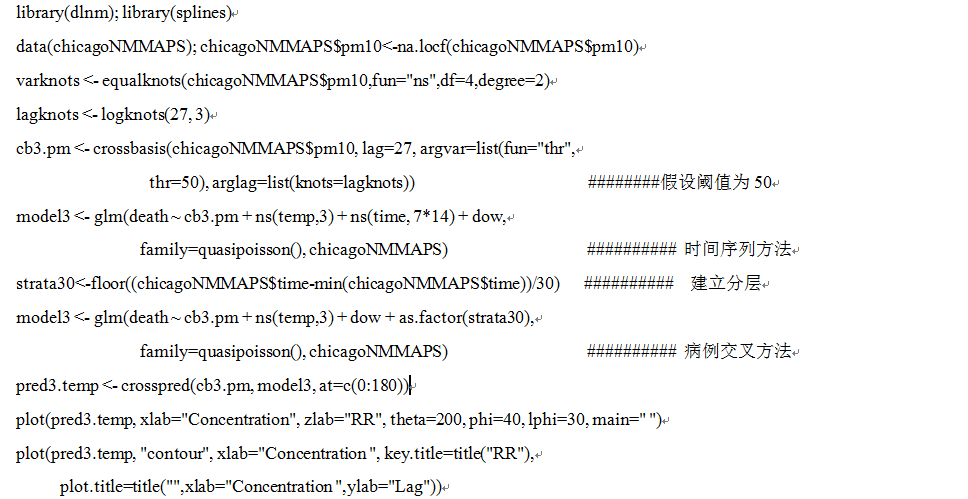
\includegraphics[width=0.8\textwidth,heigth=0.6\textwidth]{anal.png}
\end{figure}
\end{itemize}
\end{frame}

\begin{frame}{示例结果}
 \begin{figure}
 \centering
 \subfigure[3D plot]{
  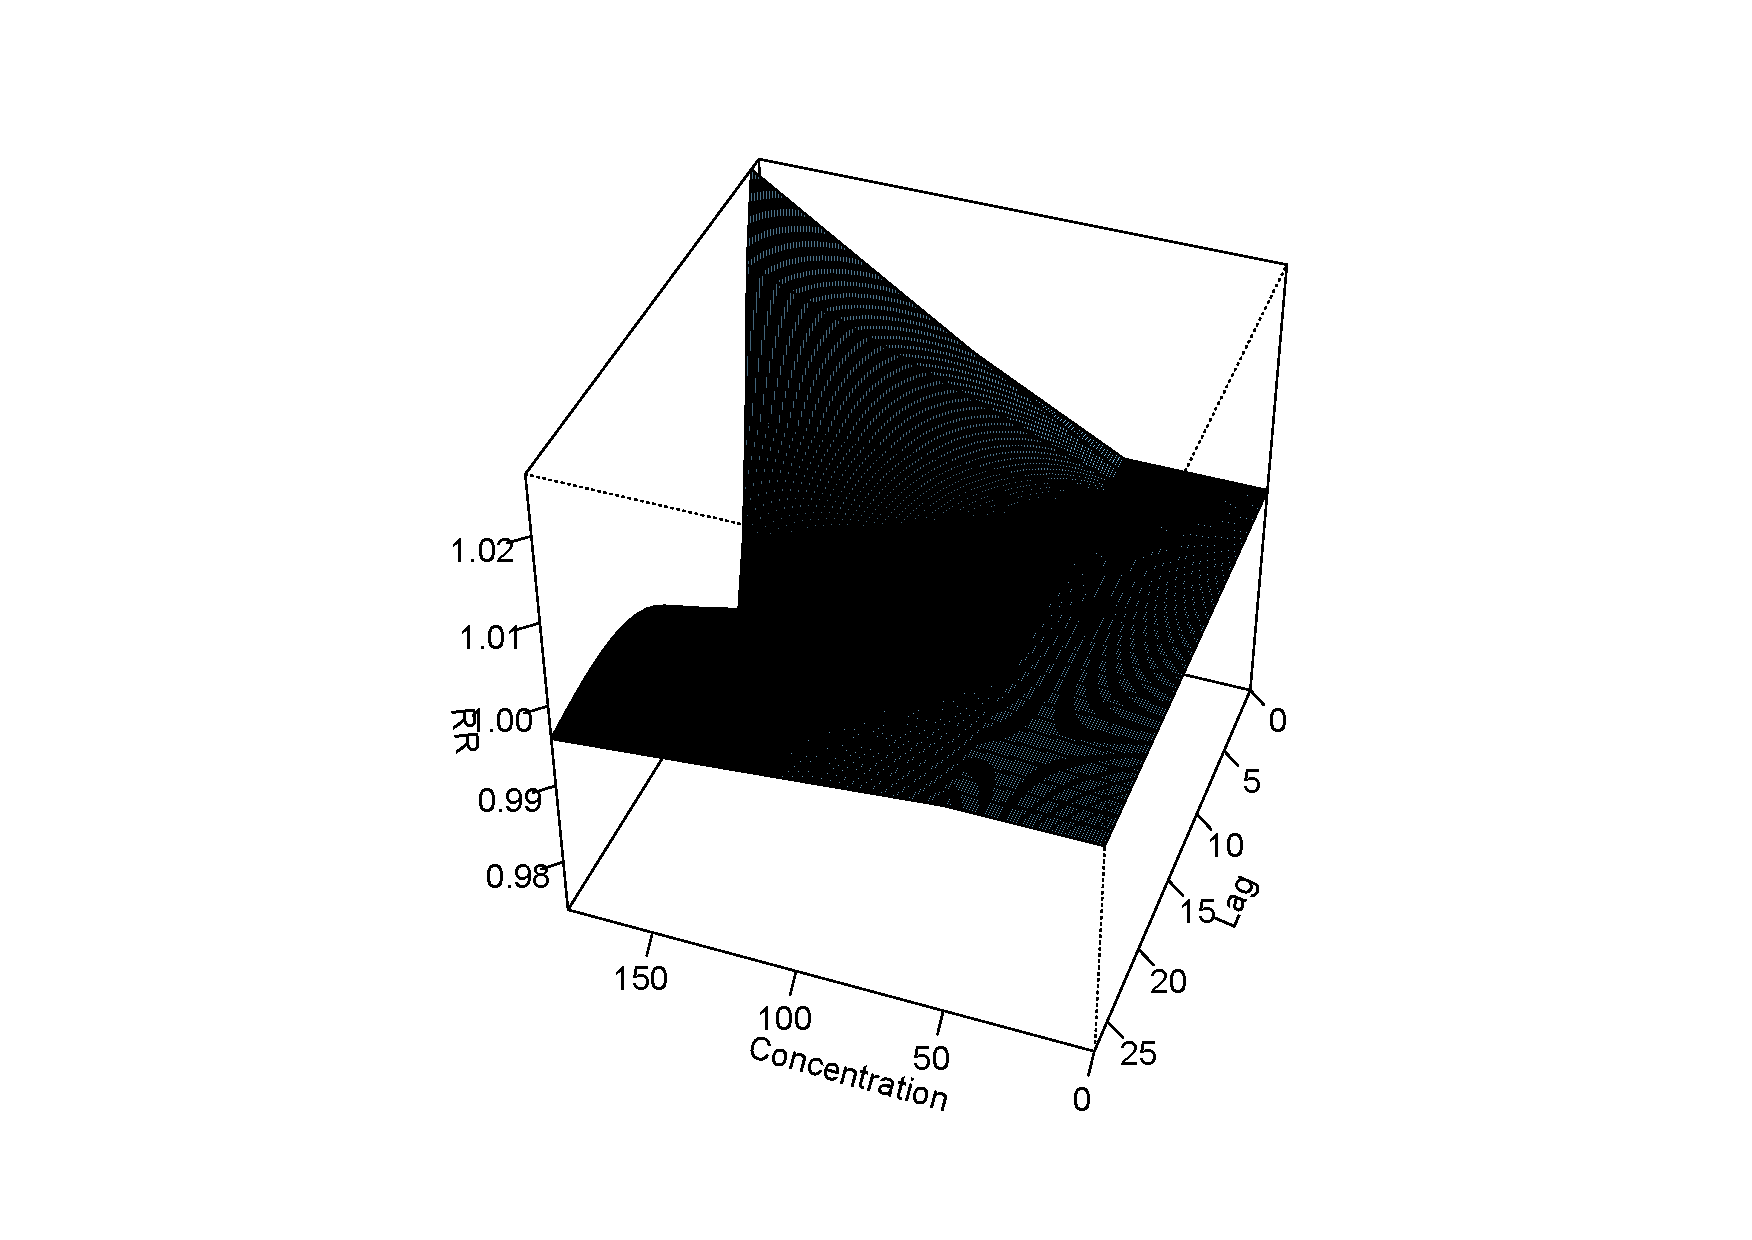
\includegraphics[width=0.45\textwidth,heigth=0.6\textwidth]{result1.pdf}
 }
 \subfigure[Contour plot]{
  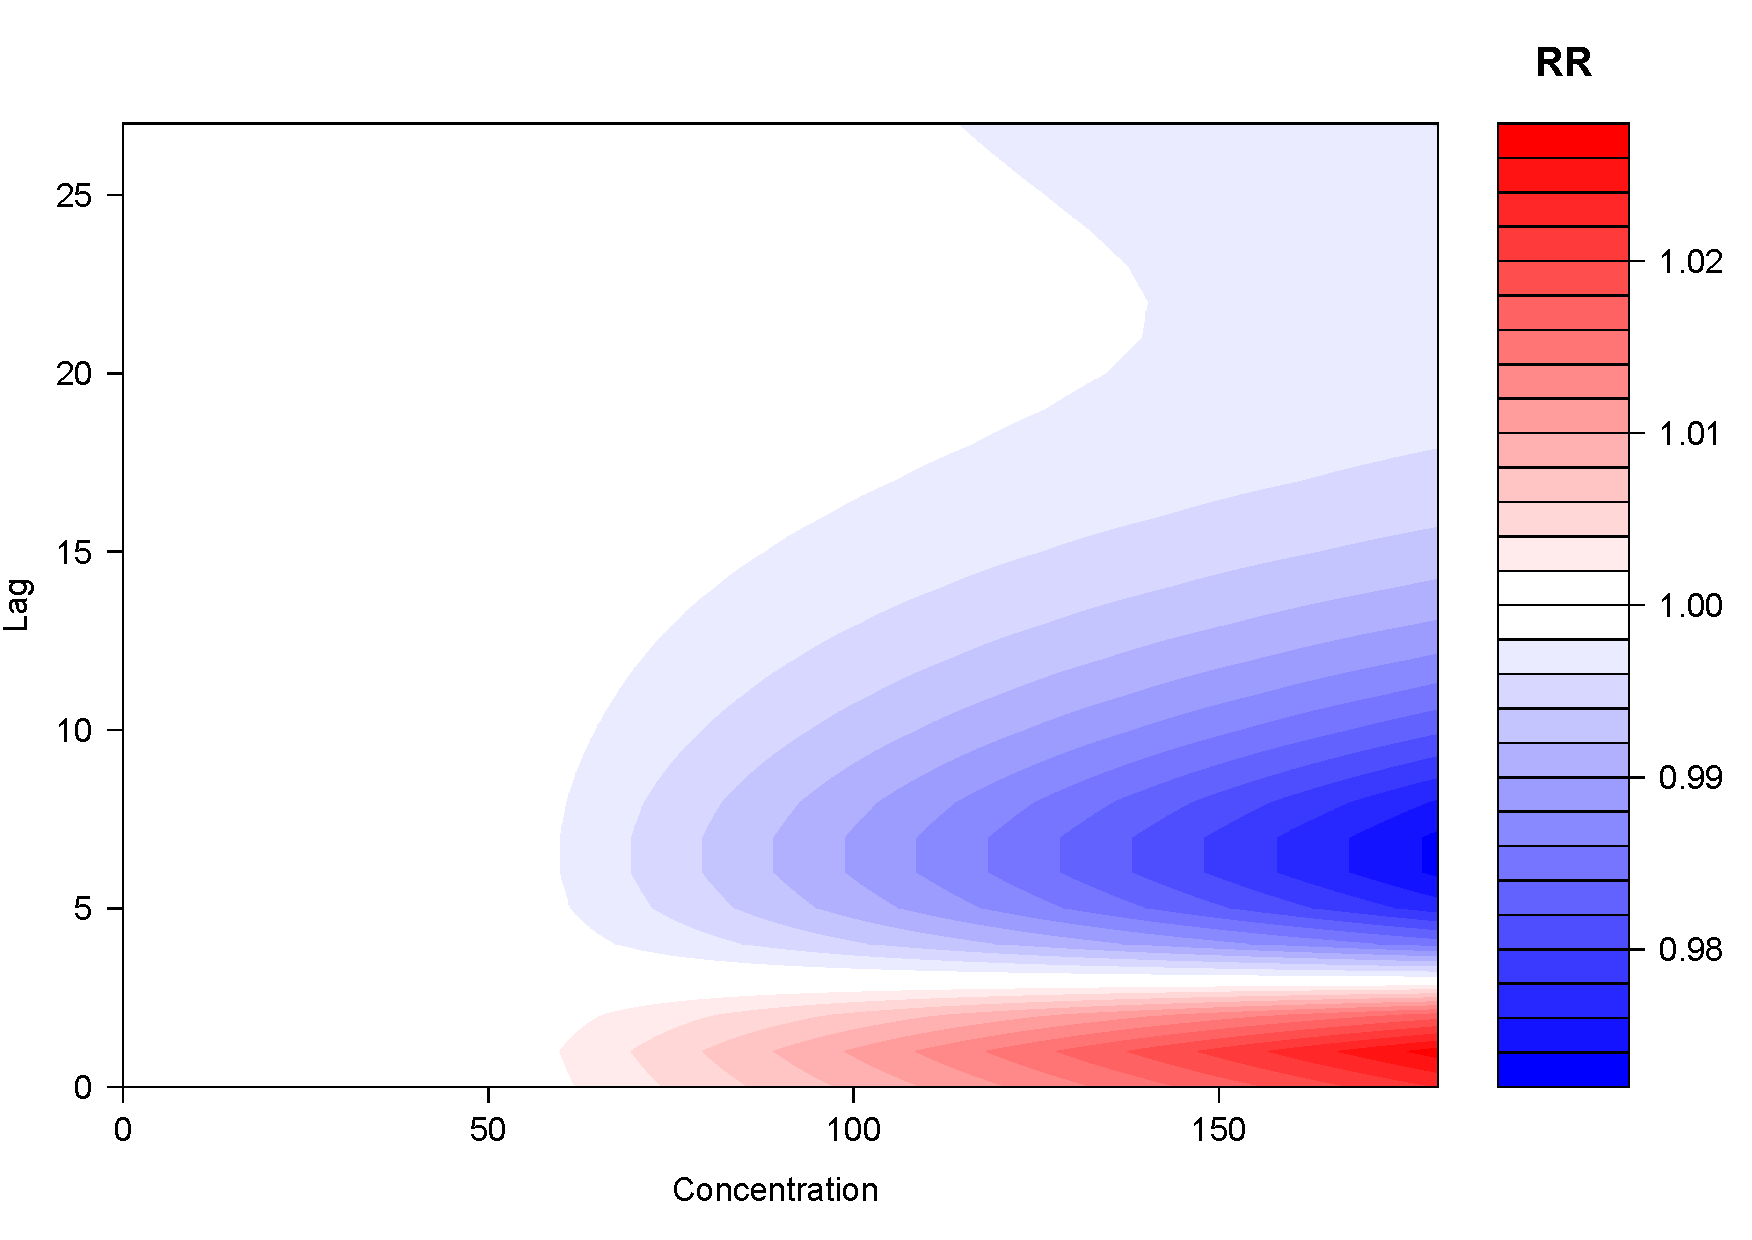
\includegraphics[width=0.45\textwidth,heigth=0.6\textwidth]{result2.pdf}
 }
 \end{figure}
 总的说来,PM$_{10}$浓度超过50$\mu$g/$m^{3}$时,相对危险度(RR)会随着PM$_{10}$浓度的升高而增大,也就是说由空气污染引发的死亡风险会增大。
\end{frame}

\section{联系作者}
% contact information
\begin{frame}{联系作者}{}
  \begin{center}
    \insertauthor\\[2ex]
	\textcolor[rgb]{0.07, 0.25, 0.62}{
    地址: 浙江省杭州滨江区滨盛路3399号\\[2ex]}
  \end{center}
\end{frame}

\end{CJK}
\end{document}
